% Drawing 141/01-12 -- folder 141, batch 01, archive page 13 (PDF page 14).
% Transcription: à droite de la suite exacte, une carte de quadrilatères accolés, à l'encre sur un premier tracé au crayon, aux sommets numérotés $0$, $1$, $2$, $3$ ; deux faces du haut sont couvertes de traits croisés au crayon.
% Kind: map of quadrilaterals with vertices numbered 0, 1, 2, 3. Method 2 (schematic redraw from the facsimile). Status: partial.
% Notes: The ink edges only, each drawn between the vertices as read, with the digits beside the vertices where he wrote them. Upper row: the quadrilateral 1-2-1-0 (top side and right side heavy, the side 0-1 heavy, one diagonal in ink) and, to its right, the quadrilateral 2-3-0-1; pencil crossed strokes in these two faces (drawn as two pencil crosses). Left: the open polygon rising from the vertex 3 at the lower left to the stroke marked 3 at the top. Lower part: the edges from the central vertex 1 to the vertices 2, 0 and 3 below it, the edges 0-1 and 2-1 to the bottom vertex 1, the heavy edge 3-2 at the left, and the detached strokes at the far left and far right. Left out: the first pencil tracing under the ink (long curved strokes across the whole figure, and an arrow to the lower right). Still differs: this is a reading of a crowded figure; several joins are uncertain (whether the thin stroke from the vertex 0 goes down to the vertex 2 below it; the strokes round the lower left vertices 3, 2, 0), some digits are hard to tell (the 1 at the top vertex, the 1 at the bottom), and which faces he meant as hatched is not settled: the note of the transcription says « certaines faces hachurées ». Redrawn 2026-11-12 (issue 128): to check again.
% Coordinates: 1 unit = 1 mm = 1/100 of the crop width (bbox in page fractions: [0.49, 0.69, 0.82, 0.885]).
% Redrawn by Claude (claude-fable-5-2), issue #128, 2026-11-12; not checked by a human; not compiled (no TeX in the session).
% Rights: reproduces part of the work -- behind RENDER_TRANSCRIPTS, never published by itself.
\documentclass[tikz,border=3pt]{standalone}
\usepackage{amsmath,amssymb}
\usetikzlibrary{patterns,arrows.meta}
\tikzset{pencil/.style={black!45}, struck/.style={black!35}, mpt/.style={circle,draw,inner sep=1.3pt}, pt/.style={circle,fill,inner sep=0.9pt}, opt/.style={circle,draw,fill=white,inner sep=1.1pt}}
\begin{document}
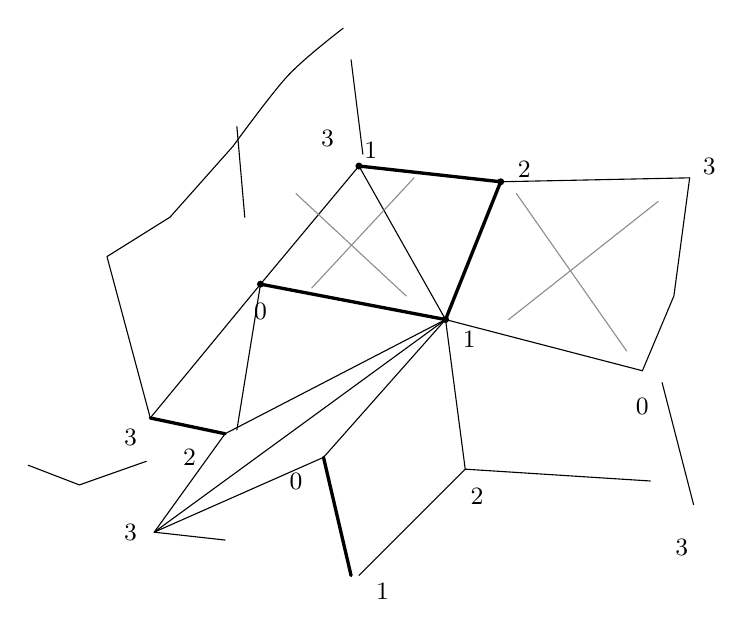
\begin{tikzpicture}[x=1mm,y=1mm,line cap=round,line join=round,font=\scriptsize]
\draw[very thick] (46,-20.5) -- (64,-22.5);
\draw[very thick] (64,-22.5) -- (57,-40);
\draw[very thick] (33.5,-35.5) -- (57,-40);
\draw (46,-20.5) -- (33.5,-35.5);
\draw (46,-20.5) -- (57,-40);
\draw (64,-22.5) -- (88,-22);
\draw (88,-22) -- (86,-37) -- (82,-46.5);
\draw (57,-40) -- (82,-46.5);
\draw (45,-7) -- (46.5,-19);
\draw plot[smooth, tension=0.55] coordinates {(44,-3) (37,-9) (30,-18)};
\draw (30.5,-15.5) -- (31.5,-27);
\draw (30,-18) -- (22,-27) -- (14,-32) -- (19.5,-52.5);
\draw[very thick] (19.5,-52.5) -- (29,-54.5);
\draw (33.5,-35.5) -- (19.5,-52.5);
\draw (33.5,-35.5) -- (30.5,-54);
\draw (29,-54.5) -- (57,-40);
\draw (57,-40) -- (41.5,-57.5);
\draw (41.5,-57.5) -- (20,-67);
\draw (57,-40) -- (20,-67);
\draw (29,-54.5) -- (20,-67);
\draw (20,-67) -- (29,-68);
\draw (57,-40) -- (59.5,-59);
\draw (59.5,-59) -- (46,-72.5);
\draw[very thick] (41.5,-57.5) -- (45,-72.5);
\draw (59.5,-59) -- (83,-60.5);
\draw (84.5,-48) -- (88.5,-63.5);
\draw (4,-58.5) -- (10.5,-61) -- (19,-58);
\draw[pencil] (38,-24) -- (52,-37);
\draw[pencil] (53,-22) -- (40,-36);
\draw[pencil] (66,-24) -- (80,-44);
\draw[pencil] (84,-25) -- (65,-40);
\node[pt] at (33.5,-35.5) {};
\node[pt] at (57,-40) {};
\node[pt] at (64,-22.5) {};
\node[pt] at (46,-20.5) {};
\node[inner sep=1pt] at (33.5,-39) {\small $0$};
\node[inner sep=1pt] at (60,-42.5) {\small $1$};
\node[inner sep=1pt] at (67,-21) {\small $2$};
\node[inner sep=1pt] at (90.5,-20.5) {\small $3$};
\node[inner sep=1pt] at (42,-17) {\small $3$};
\node[inner sep=1pt] at (47.5,-18.5) {\small $1$};
\node[inner sep=1pt] at (82,-51) {\small $0$};
\node[inner sep=1pt] at (61,-62.5) {\small $2$};
\node[inner sep=1pt] at (49,-74.5) {\small $1$};
\node[inner sep=1pt] at (87,-69) {\small $3$};
\node[inner sep=1pt] at (24.5,-57.5) {\small $2$};
\node[inner sep=1pt] at (17,-55) {\small $3$};
\node[inner sep=1pt] at (38,-60.5) {\small $0$};
\node[inner sep=1pt] at (17,-67) {\small $3$};
\end{tikzpicture}
\end{document}
